\documentclass[parskip=full]{scrartcl}
\usepackage[utf8]{inputenc} % use utf8 file encoding for TeX sources
\usepackage[T1]{fontenc}    % avoid garbled Unicode text in pdf
\usepackage[german]{babel}  % german hyphenation, quotes, etc
\usepackage{hyperref}       % detailed hyperlink/pdf configuration
\hypersetup{                % ‘texdoc hyperref‘ for options
pdftitle={SWT1: Lastenheft},%
bookmarks=true,%
}
\usepackage{graphicx}       % provides commands for including figures
\usepackage{csquotes}       % provides \enquote{} macro for "quotes"
\usepackage[nonumberlist]{glossaries}     % provides glossary commands
\usepackage{enumitem}

\makeglossaries

\title{SoftTech: iMage}
\author{Sam Weiler, 1971886}

\begin{document}

\maketitle

\section{Zielbestimmung}
Die Firma SoftTech will das neue Produkt iMage gewinnbringend vermarkten.

\section{Produkteinsatz}
Das Produkt dient zur Kunden- und Seminarverwaltung der Firma Teachware. Außerdem sollen verschiedene Anfragen beantwortet werden können.

Zielgruppe: die Mitarbeiter der Firma Teachware.

Plattform: PC mit Windows XP oder Nachfolger-Betriebssystem

\section{Funktionale Anforderungen}
\begin{itemize}[nosep]
\item[FA10] Ersterfassung, Änderung und Löschung von \glspl{Kunde} (Teilnehmer, Interessenten).
\item[FA20] Benachrichtigung der Kunden (Anmeldebestätigung, Abmeldebestätigung, Änderungsmitteilungen, Rechnung, Werbung).
\item[FA30] Ersterfassung, Änderung und Löschung von Seminarveranstaltungen und Seminartypen.
\item[FA40] Ersterfassung, Änderung und Löschung von \glspl{Dozent} sowie Zuordnung zu \glspl{Seminarveranstaltung} und \glspl{Seminartyp}.
\item[FA50] Ersterfassung, Änderung und Löschung von Seminarbuchungen.
\item[FA60] Erstellung von Rechnungen.
\item[FA70] Erhstellung verschiedener Listen (Teilnehmerliste, Umsatzliste, Teilnehmerbescheinigungen).
\item[FA80] Anfragen der folgenden Art sollen möglich sein:
     Wann findet das nächste Seminar X statt? Welche Mitarbeiter der Firma Y haben das Seminar X besucht?
\end{itemize}

\section{Produktdaten}
\begin{itemize}[nosep]
\item[PD10] Es sind relevante Daten über die Kunden zu speichern.
\item[PD20] Falls ein Kunde zu einer Firma gehört, dann sind relevante Daten über die Firma zu speichern.
\item[PD30] Es sind relevante Daten über Seminarveranstaltungen, Seminartypen und Dozenten zu speichern.
\item[PD40] Bucht ein Kunde eine Seminarveranstaltung, dann sind entsprechende Buchungsdaten zu speichern.
\end{itemize}

\section{Nichtfunktionale Anforderungen}
\begin{itemize}[nosep]
\item[NF10] Die Funktion /FA80/ darf nicht länger als 15 Sekunden Interaktionszeit benötigen, alle anderen Reaktionszeiten müssen unter 2 Sekunden liegen.
\item[NF20] Es müssen maximal 50.000 Teilnehmer und maximal 10.000 Seminare verwaltet werden können.
\end{itemize}

\section{Systemmodelle}

\subsection{Szenarien}

\subsection{Anwendungsfälle}
\subsubsection{Seminarorganisation}
\begin{center}
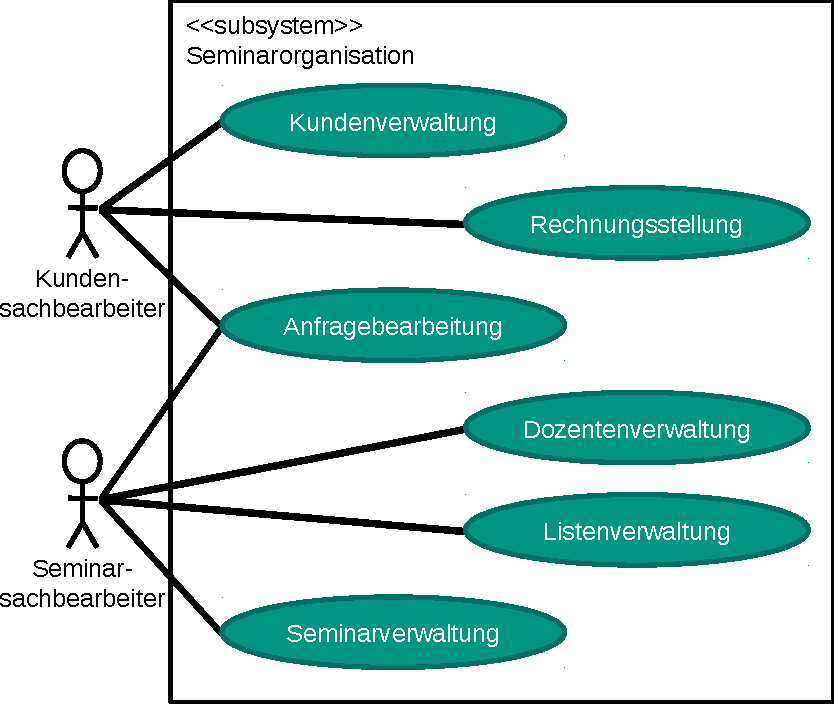
\includegraphics[width=0.8\textwidth]{szenario_seminarorganisation.pdf}
\end{center}

Akteure: Kundensachbearbeiter, Seminarsachbearbeiter.

Anwendungsfälle: Kundenverwaltung, Rechnungsstellung, Anfragebearbeitung, Dozentenverwaltung, Listenverwaltung, Seminarverwaltung.

Textuelle Beschreibung: (folgt)



%
% % Automatisch generiertes Glossar
%
%\glsaddall % das sorgt dafür, dass alles Glossareinträge gedruckt werden, nicht nur die verwendeten. Das sollte nicht nötig sein!
\printglossaries
Siehe \url{https://en.wikibooks.org/wiki/LaTeX/Glossary}.

%
% % Glossareinträge
%
\newglossaryentry{Dozent}
{
  name=Dozent,
  plural=Dozenten,
  description={Leiter eines oder mehrerer Seminartypen},
}

\newglossaryentry{Kunde}
{
  name=Kunde,
  plural=Kunden,
  description={(Zahlende) Teilnehmer einer oder mehrerer Seminarveranstaltung/en}
}

\newglossaryentry{Seminartyp}
{
  name=Seminartyp,
  plural=Seminartypen,
  description={Typ einer Lehrveranstaltung (z.B. \enquote{Schöner Malen -- Anfängerkurs})}
}

\newglossaryentry{Seminarveranstaltung}
{
  name=Seminarveranstaltung,
  plural=Seminarveranstaltungen,
  description={Tatsächlich stattfindende Lehrveranstaltung (z.B. \enquote{Schöner Malen -- Anfängerkurs, Sommer 2014})}
}

\newglossaryentry{Computer}
{
  name=Computer,
  description={Gerät zur Verarbeitung zur Daten, das die Daten einlesen, verarbeiten, speichern und ausgeben kann}
}


\end{document}
